\documentclass[spanish]{beamer}

%%% CODIFICACIÓN

%\usepackage[x11names, rgb, html]{xcolor}
\usepackage[utf8]{inputenc}
\usepackage[spanish]{babel}
\usepackage{graphics}

%%% FUENTES

\usepackage[T1]{fontenc}
\usepackage[familydefault,regular]{Chivo}
\usepackage{newtxsf} % Fuente de matemáticas
\usepackage{mathastext}
\usepackage[scaled=.85]{FiraMono}

\setbeamertemplate{navigation symbols}{}

%%% COLORES

\definecolor{50}{HTML}{FFEBEE}
\definecolor{100}{HTML}{FFCDD2}
\definecolor{200}{HTML}{EF9A9A}
\definecolor{300}{HTML}{E57373}
\definecolor{400}{HTML}{EF5350}
\definecolor{500}{HTML}{F44336}
\definecolor{600}{HTML}{E53935}
\definecolor{700}{HTML}{D32F2F}
\definecolor{800}{HTML}{C62828}
\definecolor{900}{HTML}{B71C1C}

%% Colores de Solarized

\definecolor{sbase03}{HTML}{002B36}
\definecolor{sbase02}{HTML}{073642}
\definecolor{sbase01}{HTML}{586E75}
\definecolor{sbase00}{HTML}{657B83}
\definecolor{sbase0}{HTML}{839496}
\definecolor{sbase1}{HTML}{93A1A1}
\definecolor{sbase2}{HTML}{EEE8D5}
\definecolor{sbase3}{HTML}{FDF6E3}
\definecolor{syellow}{HTML}{B58900}
\definecolor{sorange}{HTML}{CB4B16}
\definecolor{sred}{HTML}{DC322F}
\definecolor{smagenta}{HTML}{D33682}
\definecolor{sviolet}{HTML}{6C71C4}
\definecolor{sblue}{HTML}{268BD2}
\definecolor{scyan}{HTML}{2AA198}
\definecolor{sgreen}{HTML}{859900}

%% Colores del documento

\definecolor{background}{RGB}{237,237,237}
\definecolor{text}{RGB}{78,78,78}
\definecolor{accent}{RGB}{129, 26, 24}
\definecolor{accent2}{HTML}{814918}
\definecolor{accent3}{HTML}{136618}
\definecolor{accent4}{HTML}{0F4B4E}
\definecolor{accent5}{HTML}{681341}
\definecolor{accent6}{HTML}{1F1B5A}

\setbeamerfont{framesubtitle}{size=\normalfont\small}
\setbeamercolor{framesubtitle}{fg=white}

%%% AJUSTES DE BEAMER

% ¿Negrita en el título de diapositiva o no?
%\setbeamertemplate{frametitle}{\color{accent}\vspace*{1cm}\bfseries\insertframetitle\par\vskip-6pt}

\setbeamertemplate{frametitle}{\color{900}\vspace*{1cm}\insertframetitle\\\usebeamerfont{framesubtitle}\insertframesubtitle\par\vskip-6pt}

\setbeamertemplate{itemize items}[circle] % Viñetas de itemize

%%% CONFIGURACIÓN DE COLORES DE BEAMER

\setbeamercolor{background canvas}{bg=background}
\setbeamercolor{normal text}{fg=text}
\setbeamercolor{alerted text}{fg=900}
\setbeamercolor{block title}{fg=900}
\setbeamercolor{alerted text}{fg=900}
\setbeamercolor{itemize item}{fg=900}
\setbeamercolor{enumerate item}{fg=900}
\setbeamercolor*{title}{fg=900}
\setbeamercolor{qed symbol}{fg=900}
\usebeamercolor[fg]{normal text}

%%% INFORMACIÓN DEL DOCUMENTO

\title{Fundamentos de Redes}
\subtitle{Definición e implementación de un protocolo de aplicación}
\author{José María Martín Luque\\ Antonio Coín Castro\\ \vspace{1em}Grupo 2}
\begin{document}


\maketitle

\begin{frame}{Descripción de la aplicación}{Conversor de imágenes}

\begin{itemize}
	\item Paradigma cliente/servidor
    \item Cliente: usuario que envía imagen para ser convertida 
	\item Servidor: procesa imagen y realiza conversión a formato especificado
	\item Sockets TCP
\end{itemize}
\end{frame}

\begin{frame}{Diagrama de estados}{Servidor}
\begin{center}
	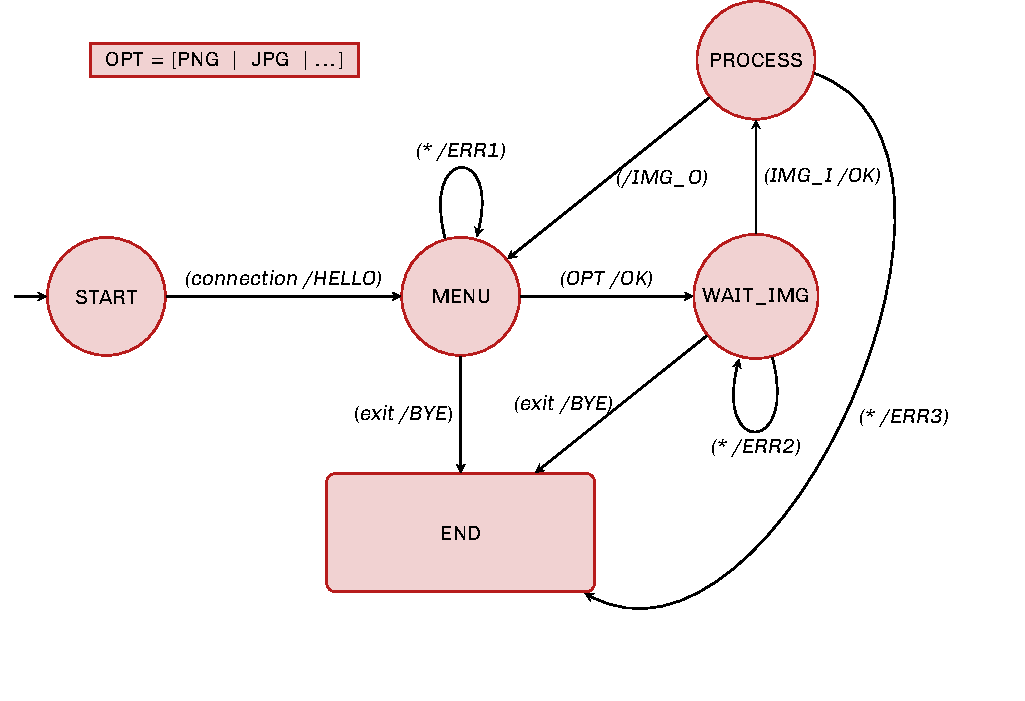
\includegraphics[width=0.85\textwidth]{img/diagrama}
\end{center}	
\end{frame}

\begin{frame}{Mensajes que intervienen}{Cliente}
\begin{center}
	\begin{tabular}{|c|c|c|}
	\hline
	Código & Cuerpo & Descripción\\
	\hline
	00 & OPT & Opción de formato a convertir\\
	\hline
	01 & IMG\_I & Datos de la imagen a convertir\\
	\hline
\end{tabular}
\end{center}
\end{frame}

\begin{frame}{Mensajes que intervienen}{Servidor}
\begin{center}
	\begin{tabular}{|c|c|c|}
	\hline
	Código & Cuerpo & Descripción\\
	\hline
	10 & HELLO & Conexión establecida\\
	\hline
	11 & OK & Datos recibidos correctamente\\
	\hline
	12 & ERR1 & Opción incorrecta\\
	\hline
	13 & ERR2 & Fallo al recibir la imagen\\
	\hline
	14 & ERR3 & Fallo al procesar la imagen\\
	\hline
	15 & IMG\_O & Imagen convertida\\
	\hline
	16 & BYE & Finalizar la conexión\\
	\hline 
\end{tabular}	
\end{center}
\end{frame}

\end{document}
